\documentclass[12pt]{beamer}
\usepackage{beamerthemeHannover, graphicx, clrscode, amsmath, amssymb, multicol}
\usepackage{textcomp}
\usepackage{verbatim}
\usepackage{listings}
\setbeamercolor{sidebar}{use=structure,bg=gray!60!green}
\lstset{language=SQL}

\title{Doing The Jitterbug \\ \small {Continuous Integration for Git} }
\author[@dukeleto]{Jonathan "Duke" Leto}
\date{}

\begin{document}

\frame{
    \titlepage
    \begin{center}
    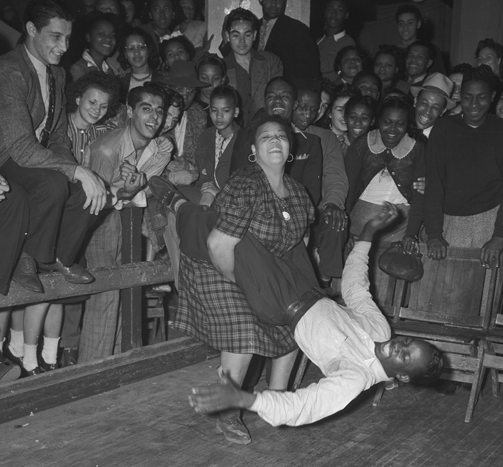
\includegraphics[width=125px, height=115px]{dancing.jpg}
    \end{center}
}

\frame{
    \frametitle{What problems does Jitterbug solve?}
    \begin{itemize}
        \item People forgetting to run the test suite
        \item People forgetting to notify others when they see breakage
        \item Not having a visual interface to which commits passed
            and which failed a test suite
    \end{itemize}
}

\frame{
    \frametitle{Current Features}
    \begin{itemize}
        \item Integrates seamlessy with Github post-receive hooks
        \item Can run tests for Perl 5/6, Parrot, Ruby and Makefile-based projects
        \item Highly customizable YAML configuration file
        \item Email notifier
        \item Supports custom build/test scripts
        \item Pretty web interface
    \end{itemize}
}


\frame{
    \frametitle{Installing/Testing Jitterbug}
    \begin{itemize}
        \item stuff
    \end{itemize}
}

\frame{
    \frametitle{Future Goals}
    \begin{itemize}
        \item stuff
    \end{itemize}
}

\frame{
    \frametitle{Get involved!}
    \begin{itemize}
        \item Jitterbug wants to support running tests in many more languages, including
        \begin{itemize}
            \item Python
            \item Javascript
            \item PHP
        \end{itemize}
        \item Submit a pull request for an issue! https://github.com/franckcuny/jitterbug
    \end{itemize}
}

\frame{
    \frametitle{ Thanks }
    \begin{itemize}
        \item stuff
    \end{itemize}
}

\frame{
    \frametitle{ Resources }
    \begin{center}
        \begin{itemize}
           \item @dukeleto / !leto on twitter/identi.ca
           \item Slides available at http://github.com/leto/presentations
        \end{itemize}
    \end{center}
}
\end{document}
